\section{Questions}

\begin{enumerate}
    \item \textbf{Définissez les termes:}
    \begin{itemize}
        \item \textbf{Approches supervisées} \\
        L'approche supervisée est utilisée quand on a un certains nombres de données connus et correctes. C'est données sont utilisées pour entrainer le modèle pour que celui-ci puisse nous 
        donner une prévision proche de la réalité. Nous avons donc appliqué une approche supervisée dans ce TP.

        \item \textbf{Approches non supervisées} \\
        Il s'agit de l'inverse de l'approche supervisée, ici on lui demande un résultat à l'aide de données aléatoires.

        \item \textbf{Régression} \\
        Utilisé pour déterminer une prédiction optimale à l'aide d'une relation linéaire entre une variable dépendante et plusieurs variables indépendantes.

        \item \textbf{Classification} \\
        Utilisé pour déterminer à qu'elle classe appartient une observation à partir de précédentes connus.

    \end{itemize}
    \item \textbf{Représenter en un schéma général, les processus d'apprentissage et de prédiction ?} \\
    \begin{figure}[!h]
        \begin{center}
            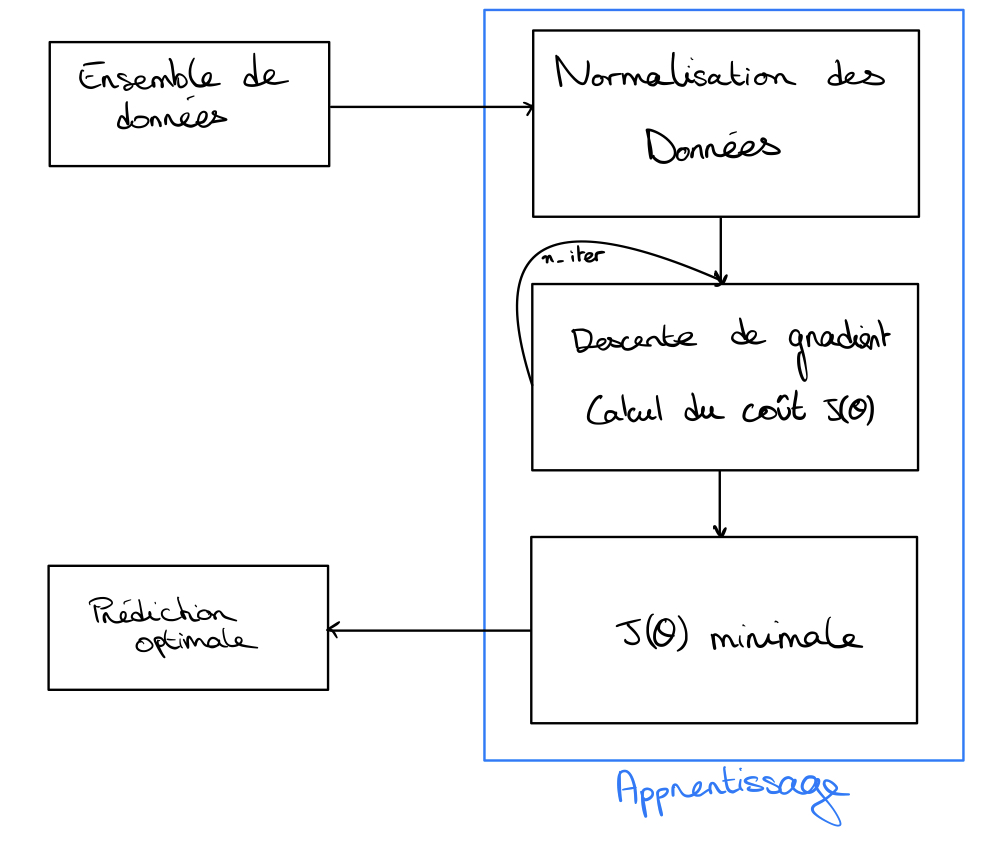
\includegraphics[width=.38\textwidth]{./img/schema.jpeg}
            \caption{\label{fig:fig6}Schéma général d'apprentissage}  
        \end{center}
    \end{figure}
    \item \textbf{Comment fonctionne l'apprentissage ? Par quels moyens ? A quoi sert la fonction de coût ? Comment est-résolu le problème ? Connaissez vous d'autres moyens de le résoudre ?} \\
    La méthode d'apprentissage par régression linéaire fonctionne grâce à l'ajustement du paramètre de notre modèle $\theta$. Pour ce faire, il faut minimiser la fonction de coût \textit{(erreur entre la prédiction et la réalité)} à l'aide
    d'une descente de gradient ce qui permet d'obtenir un $\theta$ pour réaliser une prédiction optimale. \\
    On peut résoudre ce problème avec une descente de gradient, mais également avec les équations normales.

    \item \textbf{Pourquoi faut-il parfois normaliser les descripteurs (features) ?} \\
    Il est intéressant de normaliser les données pour les ramener à une échelle commune, 
    ce qui permet d'interpréter plus facilement les résultats et rendre les calculs plus stables et rapides. Grâce à la normalisation, on peut être sûr que chaque caractéristique contribuent équitablement à la prédiction du modèle, indépendamment de son échelle initiale. \\
    
\end{enumerate}
